\documentclass[tikz,border=3mm]{standalone}

\begin{document}

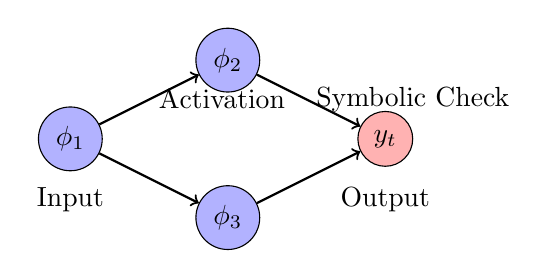
\begin{tikzpicture}
% Activation nodes
\node[circle, draw, fill=blue!30] (a) at (0,0) {$\phi_1$};
\node[circle, draw, fill=blue!30] (b) at (2,1) {$\phi_2$};
\node[circle, draw, fill=blue!30] (c) at (2,-1) {$\phi_3$};
\node[circle, draw, fill=red!30] (d) at (4,0) {$y_t$};

% Connections
\draw[->, thick] (a) -- (b);
\draw[->, thick] (a) -- (c);
\draw[->, thick] (b) -- (d);
\draw[->, thick] (c) -- (d);

% Labels
\node[below] at (0,-0.5) {Input};
\node[below] at (4,-0.5) {Output};

% Additional elements
\node[right] at (1,0.5) {Activation};
\node[right] at (3,0.5) {Symbolic Check};
\end{tikzpicture}

\end{document}
